% Copyright 2019 Clara Eleonore Pavillet

% Author: Clara Eleonore Pavillet
% Description: This is an unofficial Oxford University Beamer Template I made
% from scratch. Feel free to use it, modify it, share it.
% Version: 1.0

\documentclass[10pt]{beamer}
% Load Packages
\usepackage[utf8]{inputenc}
\usepackage{xcolor}
\usepackage{tikz}
\usetikzlibrary{positioning,calc}
\usepackage{graphicx}
\usepackage{hyperref}
\usepackage{amsmath}
\usepackage{listings}
\usepackage{fontawesome}
\usepackage[french]{babel}

% Define Commands
\newcommand*{\ClipSep}{0.06cm} %To adjust footer logo
\newcommand{\E}{\mathrm{e}\,} %\def\I{e} % used to defined e for exp(x),
% see later what it should be
\newcommand{\ud}{\mathrm{d}}
\lstset{numbers=left, numberstyle=\tiny, stepnumber=1,firstnumber=1,breaklines=true,
    numbersep=5pt,language=Python,
    stringstyle=\ttfamily,
    basicstyle=\footnotesize,
    showstringspaces=false
}


\usetheme{oxonian}

\title{GPGPU - Parallel graph cut}
\author{Nicolas Portal - Alexandre Yvart - Geoffrey Jount}
\institute{EPITA}
\date{} %\today

\begin{document}

{\setbeamertemplate{footline}{}
\frame{\titlepage}}



%%% PROBLEM DESCRIPTION
\begin{frame}{Problem description}
\end{frame}

\begin{frame}{Problem description}
\begin{center}
    Goal : image segmentation
\end{center}
\vspace{0.5cm}
    \begin{minipage}{0.5\textwidth}
    \end{minipage}%
    \begin{minipage}{0.5\textwidth}
    \end{minipage}
\end{frame}

\begin{frame}{Problem description}
\centering
\begin{center}
    Goal : image segmentation
\end{center}
\vspace{0.5cm}
    \begin{minipage}{.5\textwidth}
        \centering
        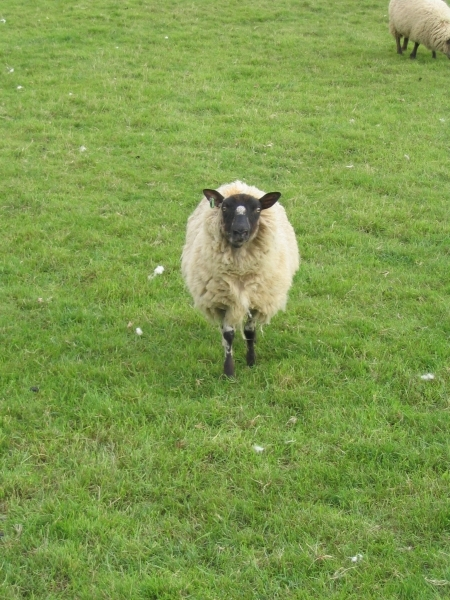
\includegraphics[width=0.8\textwidth]{input.jpg}
    \end{minipage}%
    \begin{minipage}{0.5\textwidth}
    \end{minipage}
\end{frame}

\begin{frame}{Problem description}
\centering
\begin{center}
    Goal : image segmentation
\end{center}
\vspace{0.5cm}
    \begin{minipage}{.5\textwidth}
        \centering
        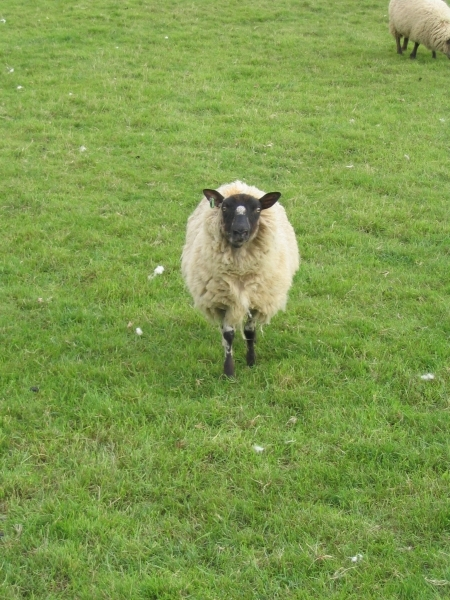
\includegraphics[width=0.8\textwidth]{input.jpg}
    \end{minipage}%
    \begin{minipage}{0.5\textwidth}
        \centering
        
\includegraphics[width=0.8\textwidth]{output.jpg}
    \end{minipage}
\end{frame}


%%% SOLUTION DESCRIPTION
\begin{frame}{Solution description}
\end{frame}

\begin{frame}{Solution description}
Push-relabel, a graph cut algorithm
\end{frame}

\begin{frame}{Solution description}
Push-relabel, a graph cut algorithm\\
$\bullet$ Manually select some foreground pixels
\end{frame}

\begin{frame}{Solution description}
Push-relabel, a graph cut algorithm\\
$\bullet$ Manually select some foreground pixels\\
$\bullet$ Manually select some background pixels
\end{frame}

\begin{frame}{Solution description}
Push-relabel, a graph cut algorithm\\
$\bullet$ Manually select some foreground pixels\\
$\bullet$ Manually select some background pixels\\
$\bullet$ Automatically find the best frontiers between foreground and
background
\end{frame}

%%% CPU IMPLEMENTATION
\begin{frame}{CPU implementation}
\end{frame}

%%% GPU IMPLEMENTATION
\begin{frame}{GPU implementation}
\end{frame}

%%% BOTTLENECKS
\begin{frame}{Bottlenecks}
\end{frame}

%%% BENCHMARKS
\begin{frame}{Benchmarks}
\end{frame}

\begin{frame}{Benchmarks}
    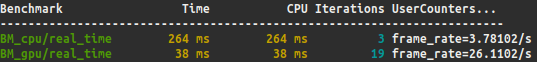
\includegraphics[width=1\textwidth]{../pics/benchmark02.png}
\end{frame}

%%% CONCLUSION
\begin{frame}{Conclusion}
\end{frame}

\begin{frame}{Conclusion}
$\bullet$ Image segmentation algorithm
\end{frame}

\begin{frame}{Conclusion}
$\bullet$ Image segmentation algorithm\\
$\bullet$ Iterative CPU
\end{frame}

\begin{frame}{Conclusion}
$\bullet$ Image segmentation algorithm\\
$\bullet$ Iterative CPU\\
$\bullet$ Parallel GPU
\end{frame}


\begin{frame}{Conclusion}
$\bullet$ Image segmentation algorithm\\
$\bullet$ Iterative CPU\\
$\bullet$ Parallel GPU\\
$\bullet$ CPU vs GPU
\end{frame}

\begin{frame}{Conclusion}
\begin{center}
    END
\end{center}
\end{frame}

\end{document}

